\subsection{Trading Framework: The Environment the Agent Trades In}
\label{Subsection:TradingFramework}

No framework was available that could both train an agent offline on quote-level history and run that same agent on a live account without rewriting it. Building one took a substantial part of the effort behind this work, and the design choices in it determine what the results in Section~\ref{Section:ExperimentalResults} are worth. Three properties were required. The tested system and the deployed system had to be the same code, so that a result obtained offline says something about live behaviour. The data had to be fine enough to reconstruct the price path inside a bar, because that path decides what a position actually paid. And the costs had to be the costs of a real account rather than a modelling convenience.

\subsubsection{System Architecture: Three Execution Contexts}

The framework is split across two languages by necessity. Strategy logic, the learning models and the market abstractions are written in Python, where the numerical and machine learning libraries are. Access to the broker is written in C\#, because cTrader \cite{noauthor_forex_nodate} executes algorithmic strategies as cBots on the .NET runtime and offers no other route to its order book. The two halves communicate through named memory-mapped files with paired auto-reset event handles, one pair for each direction, operating as a single-slot request and response exchange: the platform writes an update and signals, Python reads it, writes an action and signals back, and the platform proceeds. Two message families cross that boundary, updates travelling from the platform to Python and actions travelling the other way. Figure~\ref{Figure:SystemArchitecture} shows the arrangement. What matters is not the transport but the consequence of it: the strategy object is unaware of where its updates originate. The same class, holding the same weights, runs in three contexts.

\begin{figure}[htb!]
\centering
\begin{tikzpicture}[
  node distance=6mm,
  box/.style={draw, rounded corners=2pt, align=center, font=\small, minimum height=8mm, inner sep=3pt},
  wide/.style={box, text width=34mm},
  narrow/.style={box, text width=26mm},
  lbl/.style={font=\scriptsize\itshape},
  flow/.style={-stealth, thick},
  dashflow/.style={-stealth, thick, dashed}
]
\node[wide] (broker) {Broker\\\scriptsize IC Markets, raw spread, swap-free};
\node[wide, below=of broker] (platform) {cTrader platform};
\node[wide, below=of platform] (cbot) {Connector cBot\\\scriptsize C\# / .NET};
\node[narrow, right=14mm of cbot] (bridge) {Shared memory\\\scriptsize updates $\rightarrow$\\\scriptsize $\leftarrow$ actions};
\node[wide, right=14mm of bridge] (library) {Python library};
\node[narrow, above=8mm of library] (market) {Market abstractions\\\scriptsize ticks, bars, indicators};
\node[narrow, above=8mm of market] (strategy) {Strategy\\\scriptsize DDPG agent};
\node[narrow, below=8mm of library] (portfolio) {Portfolio\\\scriptsize orders, positions, costs};
\node[wide, below=14mm of cbot] (database) {Market database\\\scriptsize PostgreSQL, quote level};

\draw[flow] (broker) -- (platform);
\draw[flow] (platform) -- (cbot);
\draw[flow] (cbot) -- (bridge);
\draw[flow] (bridge) -- (library);
\draw[flow] (library) -- (market);
\draw[flow] (market) -- (strategy);
\draw[flow] (library) -- (portfolio);
\draw[flow] (platform.east) to[out=0, in=90] (bridge.north);
\draw[dashflow] (database) -| (library);
\node[lbl, below=1mm of database] {offline replay bypasses the platform};
\end{tikzpicture}
\caption{Framework architecture. The strategy receives updates and returns actions without knowing whether they originate from a live account, from the platform's own backtester, or from the stored quote database.}
\label{Figure:SystemArchitecture}
\end{figure}

In the first context the platform is absent. Python replays stored quotes directly from the market database, which is the fastest of the three and the one used for training and for every result reported in this work. In the second the strategy runs inside cTrader's own backtesting tab against the platform's historical data, which serves as an independent check on the offline engine. In the third the same strategy runs on a live account, receiving real quotes and sending real orders. The value of this arrangement is that the three contexts differ only in the source of the updates. A strategy that behaves one way in a backtest and another when deployed is usually the product of two separate implementations that drifted apart; here there is one implementation, and the question does not arise.

\subsubsection{Market Data: Collection, Storage and Resolution}

The historical data was collected through the same connector, requested from cTrader by the C\# component and written to a local PostgreSQL database by the Python one. Two record types are stored. Ticks hold the bid and ask quoted at an instant, together with the conversion rates needed to express a profit or loss in the account currency at that instant. Bars hold open, high, low and close as references to the ticks that produced them, so a bar is a view over the tick tape rather than a separate copy of the prices. Table~\ref{Tables:DataInventory} gives the inventory for the seven pairs. The tick tape is the primary record and the bar series are derived from it, which is what allows the engine to reconstruct the path a price took inside a bar rather than interpolating between its endpoints.

\begin{table}[htb!]
\centering
\footnotesize
\begin{tabular}{@{}lrrrrr@{}}
\toprule
\textbf{Pair} & \textbf{Ticks} & \textbf{M1 bars} & \textbf{H1 bars} & \textbf{D1 bars} & \textbf{MN1 bars} \\
\midrule
AUD/USD & 227,914,614 & 4,643,990 & 78,320 & 3,346 & 150 \\
EUR/USD & 242,847,954 & 4,636,138 & 78,145 & 3,339 & 150 \\
GBP/USD & 281,490,557 & 4,648,216 & 78,311 & 3,339 & 150 \\
NZD/USD & 203,788,307 & 4,631,614 & 78,282 & 3,339 & 150 \\
USD/CAD & 228,356,007 & 4,635,179 & 78,319 & 3,347 & 150 \\
USD/CHF & 194,186,979 & 4,621,503 & 78,307 & 3,338 & 150 \\
USD/JPY & 284,430,458 & 4,638,775 & 78,151 & 3,338 & 150 \\
\midrule
\textbf{Total} & \textbf{1,663,014,876} & \textbf{32,455,415} & \textbf{547,835} & \textbf{23,386} & \textbf{1,050} \\
\bottomrule
\end{tabular}
\caption{Market data collected from cTrader and stored locally, spanning January 2014 to August 2026. The tick tape occupies 295 GB and is the primary record; the bar series reference the ticks that produced them.}
\label{Tables:DataInventory}
\end{table}

Two properties of this data need stating, because both would otherwise look like defects.

Bars are stamped at the close of the broker's trading session rather than at midnight, at 22:00 UTC or 21:00 under daylight saving. A daily series therefore carries five bars in a normal week, stamped Sunday through Thursday, and the bar stamped Thursday is Friday's session. An audit against a calendar-day reference reports every Friday as missing, which is a convention rather than a loss. The period from 11 to 25 January 2016 is absent from all seven pairs, in ticks and in bars alike. The gap is broker-side and was confirmed unrepairable by a re-download that visited those days and returned nothing. It is uniform across the seven pairs, so it does not bias any comparison between them, and it falls outside the evaluation window used in Section~\ref{Section:ExperimentalResults}.

\subsubsection{Cost Model: Spread, Commission and Account Type}

The execution engine advances on ticks rather than on bar closes. A position opened during a bar is filled at a quote that existed within that bar, and a stop or target attached to it is tested against the quotes in the order they arrived. This matters for the reason given in Section~\ref{Section:RelatedWork}: a bar reports four prices and conceals the sequence in which the price visited them, and that sequence decides whether a stop was reached before a target and which spread was crossed.

The account modelled is a swap-free raw-spread retail account, and each of the three charges described in Section~\ref{Subsection:PerformanceMeasurement} is applied at the rate such an account pays. A buy is filled at the ask and a sell at the bid, both read from the tick tape at the instant of the fill, so the spread is charged by construction rather than deducted afterwards. The commission is charged on traded volume at $3.5$ points per side, which for a standard lot of $100{,}000$ units is $3.5$ units of the quote currency per side, or $7$ per round turn. The swap is zero, which on a swap-free account is not an approximation but the rate the account actually charges. Table~\ref{Tables:CostModel} lists the full configuration.

\begin{table}[htb!]
\centering
\footnotesize
\begin{tabularx}{\textwidth}{@{}llX@{}}
\toprule
\textbf{Setting} & \textbf{Value} & \textbf{Meaning} \\
\midrule
Account type & Raw spread, swap-free & An account a retail client can open, quoting the interbank spread and charging no overnight financing \\
\addlinespace
Spread & Accurate & The bid-ask difference recorded at the moment of the trade, read from the tick tape rather than assumed \\
\addlinespace
Commission & 3.5 points per side & Charged on traded volume; equivalently 3.5 units of the quote currency per standard lot per side, or 7 per round turn \\
\addlinespace
Swap & 0 points & The rate a swap-free account charges; not an approximation \\
\addlinespace
Account currency & EUR & Profit and loss converted at the rate recorded on the tick that produced it \\
\addlinespace
Initial balance & 10,000 & Reported across five starting balances, as described in Section~\ref{Section:ExperimentalResults} \\
\addlinespace
Leverage & 30 & The retail limit applicable to major currency pairs \\
\addlinespace
Position mode & Netting & One net position per instrument, rather than independent hedged positions \\
\bottomrule
\end{tabularx}
\caption{Cost and account configuration applied to every evaluation reported in this work.}
\label{Tables:CostModel}
\end{table}

The decision to read the spread rather than assume it is worth defending with the data, because the assumption is common and the error it introduces is not small. Figure~\ref{Figure:SpreadOverTime} plots the monthly mean spread of each pair across the evaluation window. For EUR/USD, the most liquid pair in the market, the monthly mean ranges from $0.77$ to $13.00$ points, a factor of seventeen between the quietest month and the busiest. USD/CHF reaches $37.82$ points in January 2015, when the Swiss National Bank abandoned its floor against the Euro. Across the seven pairs the ratio between the widest and narrowest month is never below five.

\begin{figure}[htb!]
\centering
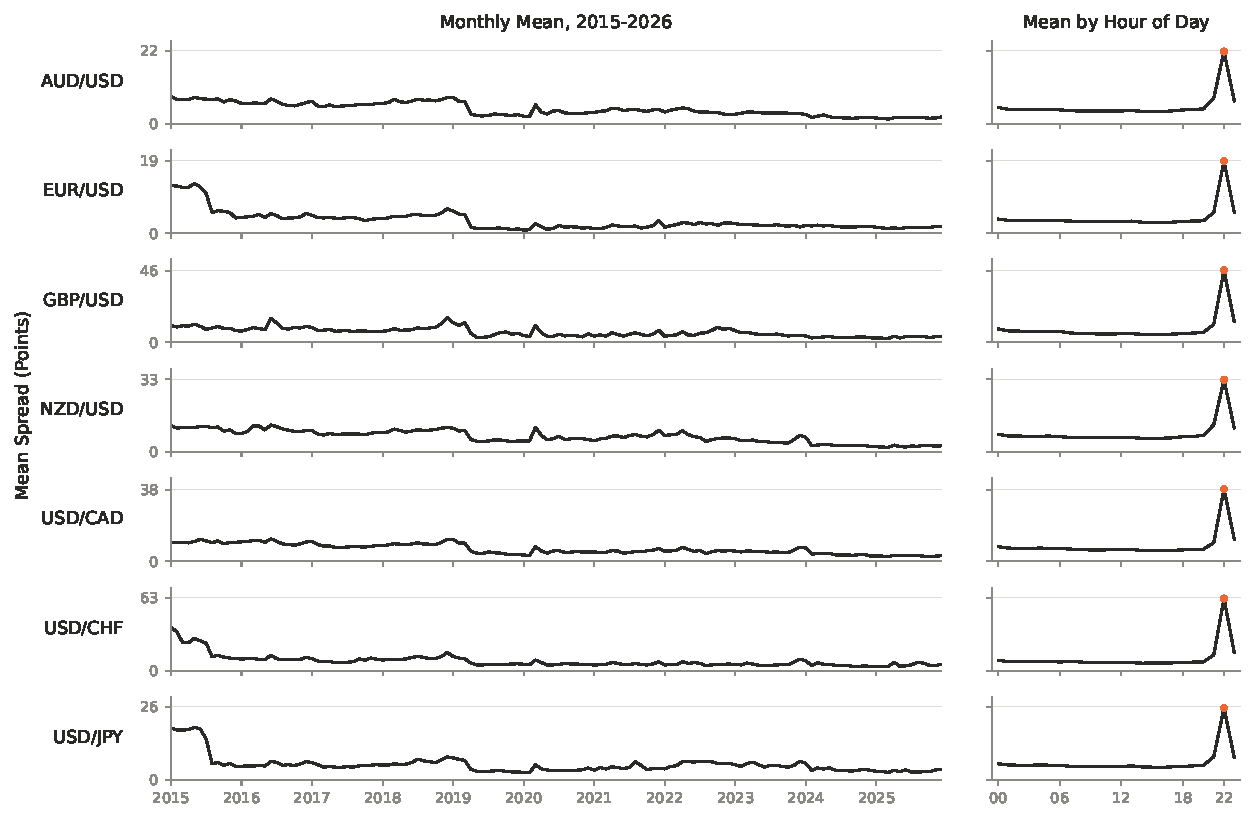
\includegraphics[width=\textwidth]{Images/SpreadOverTime.pdf}
\caption{Monthly mean spread in points for the seven major pairs, 2015 to 2026, computed from the full tick tape. EUR/USD is drawn in black. A model evaluated at a fixed spread is evaluated against a market that exists in no month of this sample.}
\label{Figure:SpreadOverTime}
\end{figure}

The shape of that variation matters more than its size. Spreads widen when liquidity falls and around the events that move prices, which are the moments at which a model trained on an average spread would most expect to act. A strategy charged a constant spread is therefore not merely charged the wrong amount; it is charged the wrong amount in a way that is correlated with its own activity, and the error runs in the direction that flatters it.

The engine was validated against cTrader's own backtester rather than against itself. Across six reference configurations, covering two currency pairs and three windows, its trade, position, order and deal records reproduce the platform's output byte for byte, and the conversion of profit and loss into the account currency was checked independently against the platform's own figures; the only divergence is sub-pip and follows from the resolution of the stored quotes rather than from the accounting. The engine therefore reproduces the platform it was built against, and then goes beyond it. The same strategy is evaluated offline directly on the tick tape, at a speed the platform's own backtester cannot reach and over windows it will not span, under a cost model that can be set to any account the broker offers rather than to the one the terminal happens to be connected to.

Two consequences follow, and both are stated here so that Section~\ref{Section:ExperimentalResults} can be read correctly. The returns reported in this work are net of the spread actually quoted and of a real commission schedule, so they are lower than the same policy would show on bar closes with a fixed or absent spread, and they are not directly comparable with results obtained that way. And because the account is swap-free, no financing term is estimated or omitted; a strategy that holds positions across many nights is charged for exactly what such an account would charge it.